\documentclass{patmorin}
\listfiles
\usepackage{pat}
\usepackage{paralist}
\usepackage{dsfont}  % for \mathds{A}
\usepackage[utf8x]{inputenc}
\usepackage{skull}
\usepackage{paralist}
\usepackage{graphicx}
\usepackage[noend]{algorithmic}

\usepackage[normalem]{ulem}
\usepackage{cancel}
\usepackage{enumitem}

\usepackage{todonotes}

% etoolbox allows for robust commands that don't need \protect, e.g.
% \newrobustcmd{\onesub}{\mathord{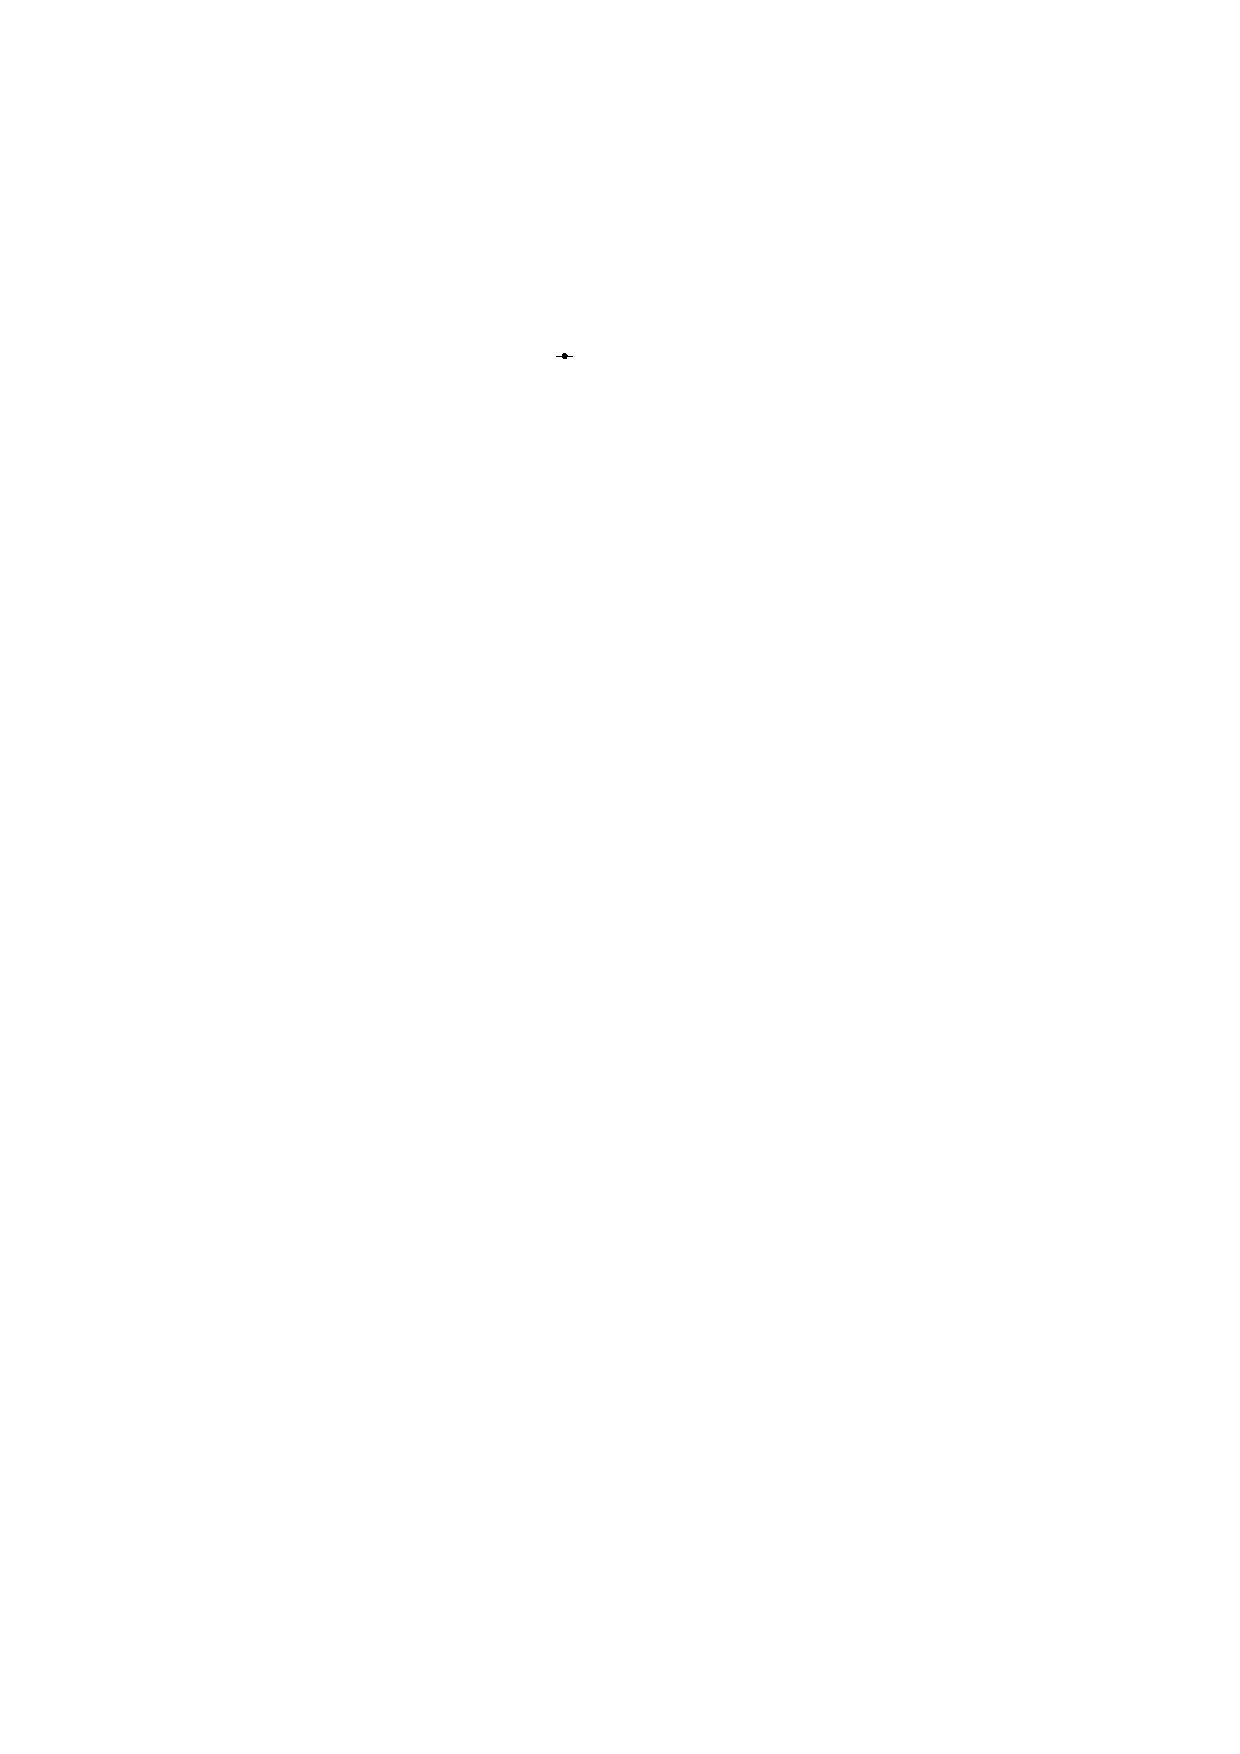
\includegraphics{figs/one-sub}}}
% \subsection{Approximate Voronoi Diagrams in $G^{\onesub}_k$}
\usepackage{etoolbox}

\usepackage[longnamesfirst,numbers,sort&compress]{natbib}

\usepackage[mathlines]{lineno}
\setlength{\linenumbersep}{2em}
% \linenumbers
% \rightlinenumbers
% \linenumbers
\newcommand*\patchAmsMathEnvironmentForLineno[1]{%
 \expandafter\let\csname old#1\expandafter\endcsname\csname #1\endcsname
 \expandafter\let\csname oldend#1\expandafter\endcsname\csname end#1\endcsname
 \renewenvironment{#1}%
    {\linenomath\csname old#1\endcsname}%
    {\csname oldend#1\endcsname\endlinenomath}}%
\newcommand*\patchBothAmsMathEnvironmentsForLineno[1]{%
 \patchAmsMathEnvironmentForLineno{#1}%
 \patchAmsMathEnvironmentForLineno{#1*}}%
\AtBeginDocument{%
\patchBothAmsMathEnvironmentsForLineno{equation}%
\patchBothAmsMathEnvironmentsForLineno{align}%
\patchBothAmsMathEnvironmentsForLineno{flalign}%
\patchBothAmsMathEnvironmentsForLineno{alignat}%
\patchBothAmsMathEnvironmentsForLineno{gather}%
\patchBothAmsMathEnvironmentsForLineno{multline}%
}


% Taken from
% https://tex.stackexchange.com/questions/42726/align-but-show-one-equation-number-at-the-end
\newcommand\numberthis{\addtocounter{equation}{1}\tag{\theequation}}


\setlength{\parskip}{1ex}

% Document-specific commands and math operators
\DeclareMathOperator{\tw}{tw}
\DeclareMathOperator{\chicen}{\chi_{\mathrm{cen}}}
\DeclareMathOperator{\chilin}{\chi_{\mathrm{lin}}}
\DeclareMathOperator{\dist}{dist}
\DeclareMathOperator{\vor}{Vor}

\newrobustcmd{\onesub}{\mathord{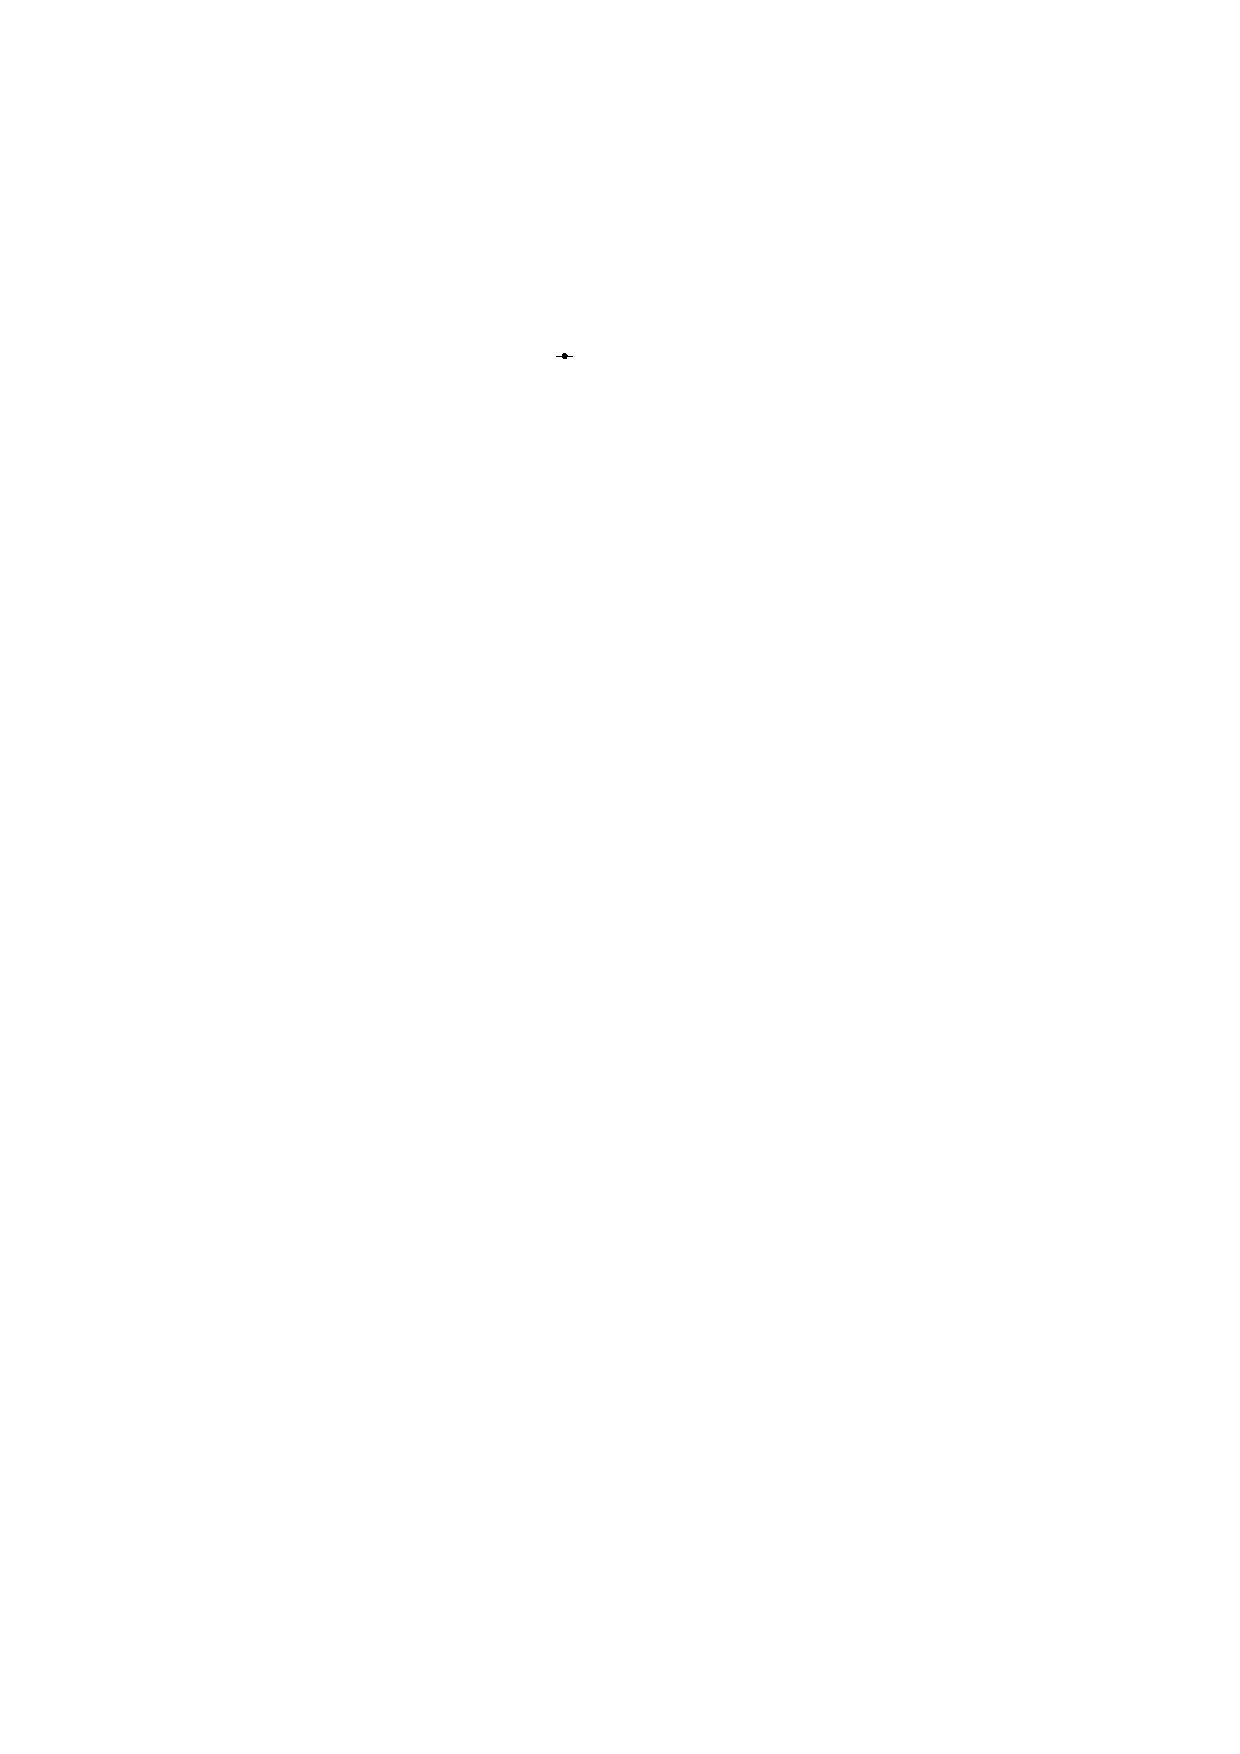
\includegraphics{figs/one-sub}}}
\newrobustcmd{\leftup}{\mathord{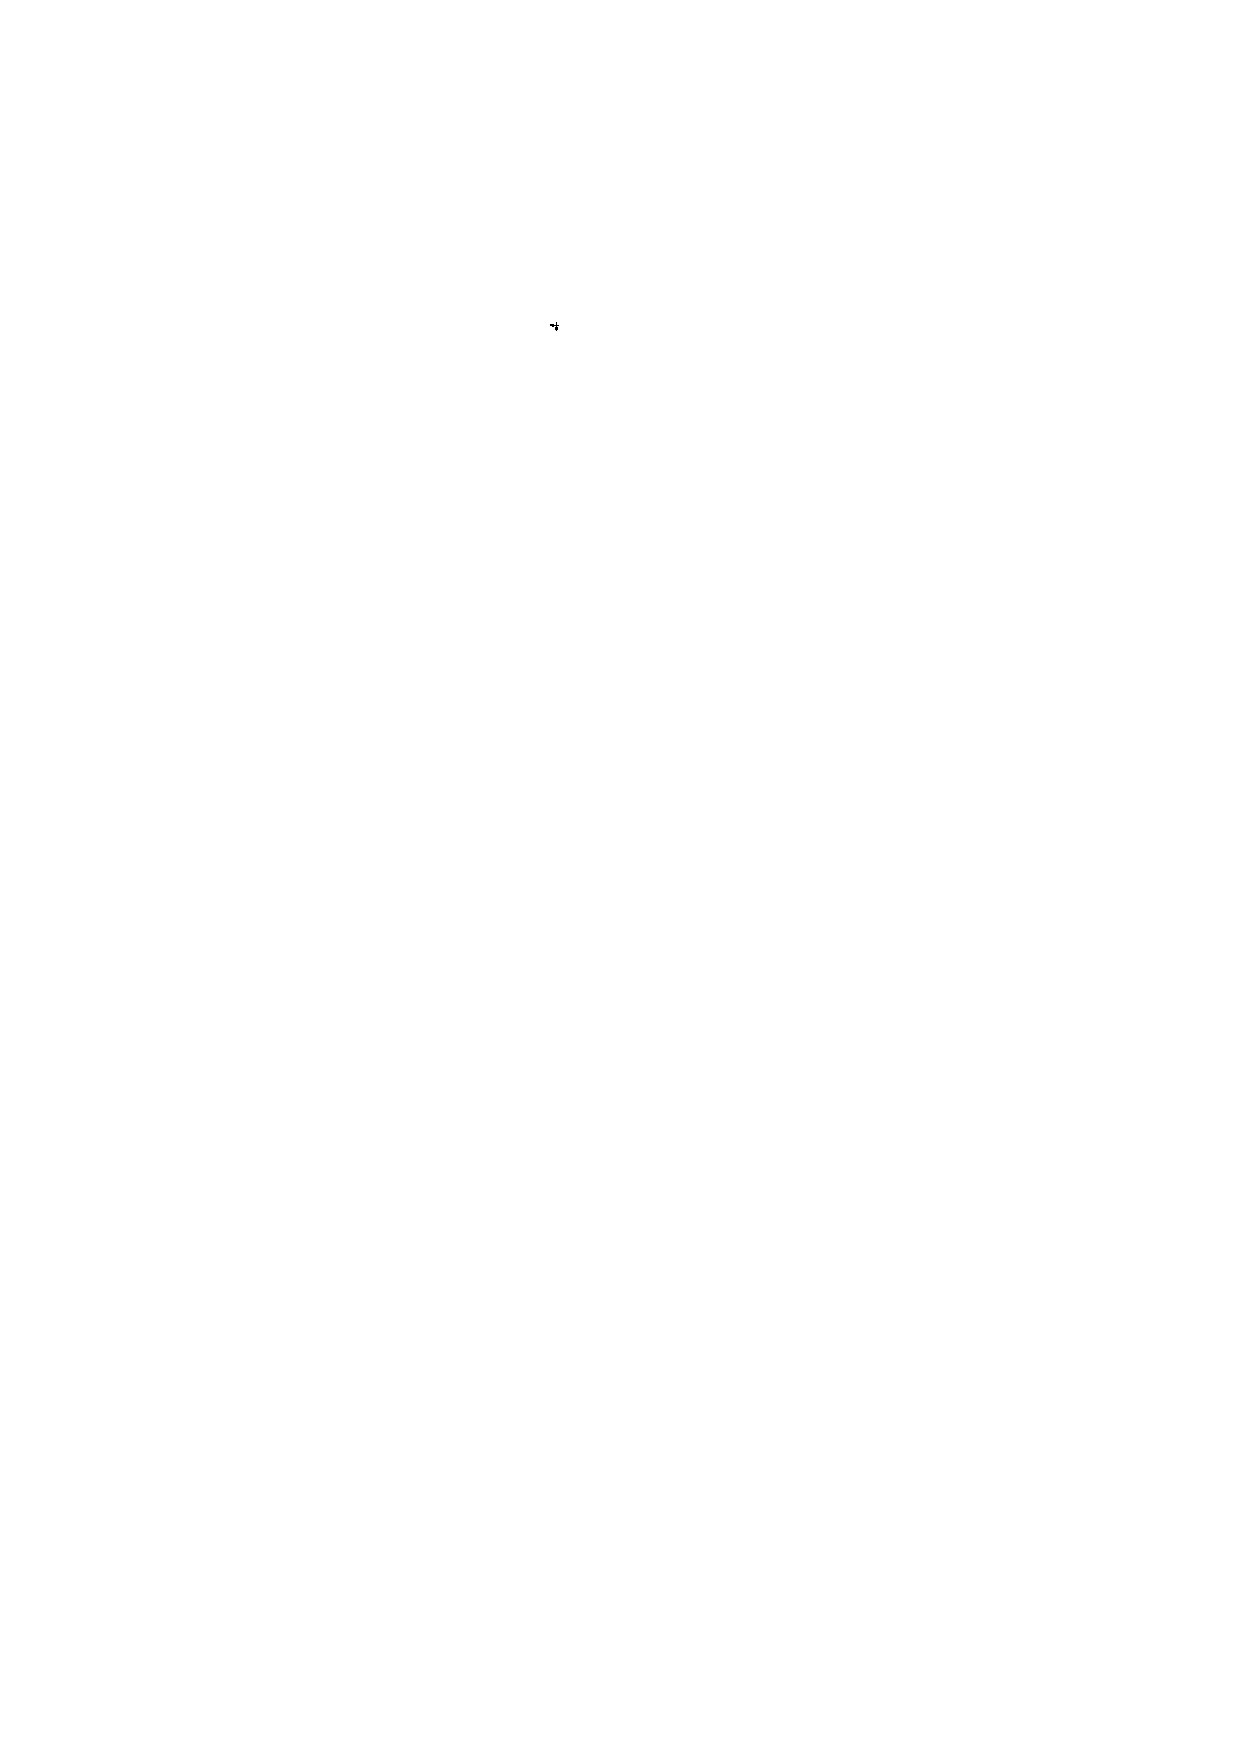
\includegraphics{figs/left-up}}}

\title{\MakeUppercase{Linear versus centred Colouring Numbers}\thanks{This research was partly funded by NSERC.}}
\author{Prosenjit Bose, Vida Dujmović, Mehrnoosh Javarsineh, and Pat Morin}

\date{}


\begin{document}

\maketitle

\begin{abstract}
    These are some notes on the relationships betwee linear colouring numbers and centred colouring numbers.
\end{abstract}

\section{Introduction}

Let $G$ be a simple undirected graph.  A \emph{$k$-colouring} of $G$ is any function $\varphi:V(G)\to S$ where $S$ is a set of size $k$.  A vertex $v$ of $G$ is a \emph{centre} of $G$ with respect to $\varphi$ if $\varphi(v)\not\in\{\varphi(w):w\in V(G)\setminus\{v\}\}$, i.e., $v$ is the unique vertex of $G$ having colour $\varphi(v)$.  A colouring $\varphi$ of $G$ is \emph{centred} if every connected subgraph of $G$ has a centre with respect to $\varphi$. A colouring $\varphi$ of $G$ is \emph{linear} if every simple path in $G$ has a centre with respect to $\varphi$.

The \emph{centred chromatic number} $\chicen(G)$ of $G$ is the minimum integer $c$ such that $G$ has a centred $c$-colouring.  The \emph{linear chromatic number} of $G$ is the minimum integer $\ell$ such that $G$ has a linear $\ell$-colouring.  Since every path in $G$ is a connected subgraph of $G$, every centred colouring of $G$ is also a linear colouring of $G$, so $\chilin(G)\le\chicen(G)$.

The question of upper bounding $\chicen(G)$ by some function of $\chilin(G)$ was considered by \citet[Theorem~1]{kun.obrien.ea:polynomial} who showed the following result:

\begin{thm}[\citet{kun.obrien.ea:polynomial}]\label{kun_obrien_general}
  For any graph $G$, $\chicen(G)\le \chilin^{190}(G)\cdot\log^{O(1)}(\chilin(G))$.
\end{thm}


Their proof of \cref{kun_obrien_general} has three steps:
\begin{enumerate}
  \item A theorem of \citet{kawarabayashi.rossman:polynomial} shows that, if $\chicen(G)\ge k^{190}\log^{O(1)} k$ then $\chilin(G)\ge k^{38}$ or $G$ has treewidth $\tw(G)\ge k^{38}$.  In the former case there is nothing left to prove.
  \item The current-best version of the Excluded Grid Theorem due to \citet{chuzhoy:improved} shows that, if $\tw(G)\ge k^{38}$, then $G$ contains an $\Omega(k^2\times k^2)$ grid minor.
  \item A technical lemma \cite[Lemma~5]{kun.obrien.ea:polynomial} shows that, if $G$ contains a $k^2\times k^2$ grid minor, then $\chilin(G)\in\Omega(k)$.
\end{enumerate}

These notes are an attempt to improve the bound in \cref{kun_obrien_general} in the general case as well as for some special classes of graphs.

As a first step, we attempt to improve the third part of the argument to show that, if $G$ contains a $k\times k$ grid minor, then $\chilin(G)\in \Omega(k)$.  This, by itself, reduces the exponent in \cref{kun_obrien_general} from $190$ to $95$.  Next, we observe that the first two parts of the argument are both ``heavy hammers'' and that, for some special graph classes, much lighter hammers suffice.  For example, if we consider only planar graphs, then it is well known that any planar graph $G$ of treewidth $k$ contains an $\Omega(k\times k)$ grid minor.  This already reduces the exponent further (for planar graphs) to $5$.  If one could prove a similar result for the first ``heavy hammer'' then this would show that, for any planar graph $G$, $\chicen(G)\in O(\chilin(G))$.


\section{Preliminaries}

For a graph $G$ and a vertex $v\in V(G)$, $\deg_G(v):=|\{vw\in E(G)\}|$ denotes the degree of $v$ in $G$.  For a any $S\subseteq V(G)$, $\deg_G(S):=\sum_{v\in S}\deg_G(v)$ is the total degree of $S$.\todo{Surely this next lemma is well-known?}

\begin{lem}\label{hall_vees}
  Let $G$ be a bipartite graph with vertex parts $A$ and $B$ and having the property that, for any $A_0\subseteq A$, $|N_G(W)|\ge 2|A_0|$.  Then $G$ contains a subgraph $\Lambda$ in which each vertex of $A$ has degree exactly two and each vertex of $B$ has degree at most one.
\end{lem}

\begin{proof}
  Let $\Lambda$ be a subgraph of $G$ in which each vertex of $A$ has degree at most two, each vertex of $B$ has degree at most one, and that maximizes $\deg_\Lambda(A)$.  If $\deg_{\Lambda}(A) = 2|\Lambda|$ then there is nothing to prove. Assume therefore, for the sake of contradiction,  that there exists $v_0\in A$ with $\deg_\Lambda(v_0) < 2$.

  We say that a path $v_0,\ldots,v_m$ in $G$ is \emph{$\Lambda$-aternating} if $v_iv_{i+1}\in E(\Lambda)$ for all odd $i\in\{0,\ldots,m-1\}$ and $v_iv_{i+1}\not\in E(\Lambda)$ for all even $i\in\{0,\ldots,m\}$.  Observe that any such path has even length so that it ends at a vertex $v_m\in A$.  Otherwise, replacing the edges $\lfloor m/2\rfloor$ edges $\{v_1v_2,v_3v_4,\ldots,v_{m-2}v_{m-1}\}\in E(\Lambda)$ with the $\lceil m/2\rceil$ edges $\{v_0v_1,v_2v_3,\ldots,v_{m-1}v_m\}$ does not change $\deg_\Lambda(v)$ for any $v\in A_0\setminus\{v_0\}$ but does increase  $\deg_\Lambda(v_0)$, contradicting the assumption that $\Lambda$ maximizes $\deg_\Lambda(A)$.

  Let $A_0\subseteq A$ and $B_0\subseteq B$ be the subsets of $A$ and $B$, respectively, that can be reached from $v_0$ by $\Lambda$-alternating paths.
  Observe that, for any $x\in B_0$,  there is exactly one edge $vx$ of $\Lambda$ incident on $x$ and the other endpoint $v$ of this edge is in $A_0$.  Let $a$ be the number of edges of $\Lambda$ having one endpoint $A_0$ and one endpoint in $B_0$, so that $a=\deg_\Lambda(B_0)=|B_0|$.  Let $b$ be the number of edges of $\Lambda$ having one endpoint in $A_0$ and one endpoint in $B\setminus B_0$, so that $\deg_\Lambda(A_0)=a+b = |B_0|+b$.    Since $\deg_{\Lambda}(v) \le 2$ for each $v\in A_0$ and $\deg_\Lambda(v_0)<2$, $\deg_\Lambda(A_0)<2|A_0|$.  This yields the desired contradiction, since $|N_\Lambda(A_0)| \le \deg_\Lambda(A_0) = |B_0|+b = \deg_\Lambda(A_0)< 2|A_0|$.
\end{proof}


\section{The Linear Colouring Number of Pseudogrids}

A \emph{subdivision} of a graph $G$ is any graph $G'$ that can be obtained from $G$ by replacing each edge $vw$ of $G$ with a path $v,s_1,s_2,\ldots,s_\ell,w$ in which each of the (newly introduced) internal vertices $s_1,\ldots,s_\ell$ have degree exactly $2$.  Each vertex in $V(G')\setminus V(G)$ is called a \emph{subdivision vertex}.  A $\ell$-subdivision of $G$ is a subdivision of $G$ in which each edge of $G$ is replaced by a path that has exactly $\ell$ internal vertices.  For a graph $G$, we use $G^{\onesub}$ to denote the $1$-subdivision of $G$.

\subsection{Subdivided Grids}

For positive integers $a$ and $b$, the \emph{$a\times b$ grid} $G_{a\times b}$ is the graph with vertex set $V(G_{a\times b}):=\{1,\ldots,a\}\times\{1,\ldots,b\}$ and that contain an edge with endpoints $(v,w)$ and $(x,y)$ if and only if $|v-x|+|w-y|=1$.  For each $i\in\{1,\ldots,a\}$, the \emph{$i$th column} of $G_{a\times b}$ is the vertex set $\{(i,1),\ldots,(i,b)\}$ and, for each $j\in\{1,\ldots,b\}$, the $j$th row is the vertex set $\{(1,j),\ldots,(a,j)\}$.  We define the \emph{boundary} of $G_{a\times b}$ as $\partial G_{a\times b}:=\{1,a\}\times\{1,\ldots,b\}\cup \{1,\ldots,a\}\times\{1,b\}$.  We say that a path $P:=v_0,v_1,\ldots,v_\ell$ in $G_{a\times b}$ \emph{goes straight} at a vertex $v_i$, $i\in\{1,\ldots,k-1\}$ if $v_{i-1}$, $v_i$, and $v_{i+1}$ are contained in a single row or column.  Otherwise, we say that $P$ \emph{turns} at $v_i$.

\begin{figure}
  \begin{center}
    \begin{tabular}{cc}
      \includegraphics{figs/grid-1} &
      \includegraphics{figs/grid-2}
    \end{tabular}
  \end{center}
  \caption{The grid $G_{10}$ and its $1$-subdivision $G^{\onesub}_{10}$.}
\end{figure}

% An $a'\times b'$ \emph{subgrid} of $G_{a\times b}$ is an induced graph of the form $G_{a\times b}[\{(v,w): v\in\{i,\ldots,i+a'-1\},\, w\in\{j,\ldots,j+b'-1\}$ for some $i\in\{1,\ldots,a-a'+1\}$ and $j\in\{1,\ldots,b-b'+1\}$.   The \emph{vertex boundary} of $G_{a\times b}$ is $\{1,a\}\times\{1,\ldots,b\}\cup \{1,\ldots,a\}\times\{1,b\}$.  The \emph{edge boundary} of $G_{a,b}$ consists of all edges incident to at least one vertex in the vertex boundary of $G_{a,b}$. The \emph{boundary} of $G_{a\times b}$ is the union of the edge and vertex boundaries.

For brevity, we use $G_{k}:=G_{k\times k}$ as a shorthand for the $k\times k$ grid.  We will work extensively with the $1$-subdivision $G^{\onesub}_k$ of $G_k$.  In this case, we define $\partial G^{\onesub}_k:=\{v\in V(G^{\onesub}_k):\dist_{G^{\onesub}_k}(v,\partial G_k)\le 1\}$.  That is, the boundary of $G^{\onesub}_k$ includes the vertex boundary of $G_k$ as well as any degree-$2$ vertex of $G^{\onesub}_k$ that is adjacent to at least one boundary vertex of $G_k$.

\begin{figure}
  \begin{center}
    \includegraphics{figs/grid-3}
  \end{center}
  \caption{The ball $B_2(v)=B_2(s)$ in $G^{\onesub}_{10}$.}
\end{figure}


\begin{lem}\label{seven_by_seven}
  Let $I,L,Q$ be disjoint subsets of $V(G^{\onesub}_{7})\setminus \partial G^{\onesub}_k$ with $|I\cup L\cup Q|\le 3$ that have the following properties:
  \begin{compactenum}[(i)]\setcounter{enumi}{0}
    \item Each vertex is $I\cup L$ has degree $4$ and each vertex in $Q$ has degree $2$.
    \item No vertex in $V(G^{\onesub}_{10})$ is adjacent to three vertices of $Q$.
    \item No vertex in $I\cup L$ is adjacent to two vertices of $Q$.
  \end{compactenum}
  Then for any pair of boundary vertices $s$ and $t$, $G_{10}$ contains a path $P$ that
  \begin{compactenum}[(a)]
    \item begins at $s$ and ends at $t$;
    \item contains every vertex in $I\cup L\cup Q$;
    \item goes straight through each vertex in $I$; and
    \item turns at each vertex in $L$.\todo{Define turns and goes straight}
    % \item contains no boundary vertices or edges except $s$ and $t$.
  \end{compactenum}
\end{lem}

\begin{proof}
  I have no idea how to prove this.  Computer search?.
\end{proof}

It will be helpful to take some natural definitions for $G_k$ and extend them to $G^{\onesub}_k$.  To do this, we associate each vertex $v$ of $G^{\onesub}_k$ with a vertex $v^{\leftup}$ of $G_k$. For each vertex $v\in V(G_k)$, we define $v^{\leftup}:=v$. For each subdivision vertex $s$ in $G^{\onesub}_k$ with neighbours $v$ and $w$, we define $s^{\leftup}$ to be the lexicographically smaller of $v$ or $w$.  For two vertices $v_1,v_2\in V(G^{\onesub}_k)$, with $v^{\leftup}_1:=(x_1,y_1)$ and $v^{\leftup}_2:=(x_2,y_2)$ we define the $L_\infty$-distance between $v_1$ and $v_2$ as $\|v_1v_2\|_\infty = \max\{|x_1-x_2|, |y_1-y_2|\}$.  For any $v\in V(G^{\onesub}_k)$, the \emph{($L_\infty$) ball} of radius $r$ centered at $v$ is $B_{r}(v):=\{w\in V(G^{\onesub}_k):\|vw\|_\infty \le r\}$.\todo{Make a figure that illustrates this.}

\begin{lem}\label{four_points}
  Let $P$ be a set of at most $3$ vertices of $G^{\onesub}_k$.  Then there exists a set $S$ of pairwise-disjoint balls, each of radius $3$, such that each vertex in $P$ is contained in the interior of some ball in $S$.\todo{Define the interior of a ball.}
\end{lem}

\begin{proof}
  Let $P:=\{v_1,\ldots,v_t\}$ where $p_i^{\leftup}:=(x_i,y_i)$.  Let $X:=\bigcup_{i=1}^t \{x_i\bmod 10,(x_{i+1})\bmod 10\}$ and let $Y:=\bigcup_{i=1}^t\{y_i\bmod 10,(y_i+1)\bmod 10\}$.  Then $|X|,|Y|\le 2t\le 6$.  In particular, there exists some $x\in\{0,\ldots,6\}\setminus X$ and some $y\in\{0,\ldots,6\}\setminus Y$. For each $i,j\in\Z$, let $c_{i,j}:=(7i+x+3,7j+y+3)$ and observe that the ball $B_{3}(c_{i,j})$ does not have any point of $P$ on its boundary.  Furthermore, the set of balls $S:=\{B_{3}(c_{i,j}):i,j\in\Z\}$ is a partition of $V(G^{\onesub}_{k})$.  Therefore $S$ is a set of pairwise-disjoint balls, each of radius $3$, such that each vertex in $P$ is contained in the interior of some ball in $S$.
\end{proof}

\begin{lem}
  Let $P$ be a subset of $V(G^{\onesub}_k)$ such that no ball of radius $9$ contains more than $3$ vertices in $P$.  Then there exists a set $S$ of disjoint balls, each of radius $3$ and such that each point of $P$ is in the interior of some ball in $S$.
\end{lem}

\begin{proof}
  Define a graph $H$ with vertex set $V(H):=P$ and that contains an edge $pq$ if and only if $\|pq\|_\infty \le 12$. Observe that, if some connected subgraph of $H$ contains $4$ vertices, then these $4$ vertices are contained in a ball of radius $9$.  Therefore each component of $H$ contains at most $3$ vertices.

  For each component $C$ of $H$, apply \cref{four_points} to $V(C)$ and keep only those balls in $S$ that contain at least one vertex of $V(C)$.  This produces a set $S_C$ of disjoint balls, each of radius $3$, that each contain some vertex in $V(C)$ in their interior.  Any two balls $B_{C_1}$ and $B_{C_2}$ obtained from different components of $H$ are disjoint because the first ball contains a vertex $p_1\in P$ and the second ball contains a vertex $p_2\in P$ such that $\|p_1p_2\|\infty > 12$, but the balls $s_1$ and $s_2$ each have radius $3$.
\end{proof}


\begin{lem}\label{one_path_enchilada}
  Let $k$ be a positive integer, let $I,L,Q$ be disjoint subsets of $V(G^{\onesub}_{k})\setminus\partial G^{\onesub}_k$ that have the following properties:
  \begin{compactenum}[(1)]\setcounter{enumi}{-1}
    \item Any ball of radius 9 contains at most $3$ elements of $I\cup L\cup Q$.
    \item Each vertex in $I\cup L$ has degree $4$ and each vertex in $Q$ has degree $2$.
    \item No vertex in $V(G^{\onesub}_{10})$ is adjacent to three vertices of $Q$.
    \item No vertex in $I\cup L$ is adjacent to two vertices of $Q$.
  \end{compactenum}
  Then $G^{\onesub}_k$ contains a path $P$ that
  \begin{compactenum}[(a)]
    \item contains all the vertices in $I\cup L\cup Q$;
    \item goes straight through each vertex in $I$; and
    \item turns at each vertex in $L$.
  \end{compactenum}
\end{lem}

\begin{proof}
  Start with the snakelike path $P_0$ that visits every $7$th row of $G_k$. Cover the elements of $I\cup L\cup Q$ with disjoint balls of side length $3$.  Each such square is intersected by exactly one row of the snakelike path.  Use \cref{seven_by_seven} to locally deform $P_0$ to pick up the objects in any square that it intersects.
\end{proof}


\subsection{Approximate Voronoi Diagrams in $G^{\onesub}_k$}

Here we explain the ranking trick that allows us to make approximate Voronoi diagrams.  If the minimum-distance between any two sites in these diagrams is $\beta$, then any four points in four different cells of the diagram contains a pair of points at distance $\Omega(\beta)$.  In particular, there exists a constant $a>0$ such that any ball of radius $a\beta$ contains points from at most $3$ grid cells.  We will then use this to find vertex sets $P\subseteq V(G^{\onesub}_k)$ that can be used with \cref{one_path_enchilada}.


% \todo[inline]{This lemma is not true. Pick a center $x$ and place a point in each of the quadrants around $x$ where the $i$th point is at distance $10\beta - (ir)$ from $x$.  Then $x$ is incident on all four Voronoi regions.  We really have to use the fact that $\beta$ (or rather, $\beta+ar$) is also an upper bound on the distance we actually care about.}
\begin{lem}
  For any $\beta, k\in\N$ and any $P\subseteq V(G^{\onesub}_k)$ with $\min\{\|pq\|_\infty:p,q\in\binom{P}{2}\} \ge \beta$ the following statement is true:  Let $Q:=\bigcup_{p\in P} B_\beta(p)$. There exists a function $\vor_P:Q\to P$ such that
  \begin{compactenum}[(i)]
    \item for any $v\in Q$, $|\{\vor_P(v)\}\cup\{\vor_P(w):w\in Q\cap N_{G^{\onesub}_k}(v)\}|\le 2$.
    \item for any ball $B$ of radius $\beta/12$, $|\{\vor_P(v):v\in B\cap Q\}|\le 3$;
  \end{compactenum}
\end{lem}

\begin{proof}
  % The idea behind this proof is to use the Voronoi diagram of $P$ to define the function $\vor$.  The problem is that the Voronoi diagram can have vertices of high degree and pairs of vertices that are close together, both of these violate the second requirement.  Instead, we construct an approximate Voronoi diagram in which each point is assigned to one of
  We first define a function $\vor':Q\to P$ that satisfies the second condition and then show how local modifications can be used to obtain a function $\vor$ that satisfies both conditions.

  Arbitrarily order the vertices of $P$ as $p_1,\ldots,p_{|P|}$.  For each $v\in Q$, let $d(v):=\min\{\|vp\|_\infty:p\in P\}$, let $S(v):=\{p\in P:\|vp\|_\infty \le d(v)+3\beta/4\}$, and let $\vor'_P(v):=\min\{i:p_i\in S(v)\}$.  In words, $d(v)$ represents the distance from $v$ to its nearest neighbour in $P$, $S(v)$ represents the set of approximate nearest neighbours of $v$ in $P$ (up to an additive error of $\beta/12$), and $\vor_P'(v)$ is (the index of) the approximate nearest neighbour of $v$ of smallest index.

  We now argue that $\vor'$ satisfies the second condition.  Let $v_1,\ldots,v_4\in Q$ and $1\le i_1<\cdots<i_4\le|P|$ be such that $\vor_P'(v_j)=i_j$ for each $j\in\{1,\ldots,4\}$.  Suppose, for the sake of contradiction, that $i_1,\ldots,i_4$ are all distinct and that $v_1,\ldots,v_4$ are contained in some ball $B_{\beta/12}(c)$.  By the triangle inequality $\|v_iv_j\|_\infty \le \|v_ic\|_\infty+\|cv_j\|_\infty \le \beta/6$ for each  $i,j\in\{1,\ldots,4\}$.
  Since $v_1\in Q$, $d(v)\le\beta$ so
  \[ \|p_{i_1}v_1\|_\infty \le d(v_1) + 3\beta/4 \le \beta + 3\beta/4 \]
  Since $\vor'(v_2)=i_2\neq i_1$,
  \[ \|p_{i_2}v_2\|_\infty
     < \|p_{i_1}v_2\|_\infty - 3\beta/4
     \le \|p_{i_1}v_1\|_\infty + \beta/6 - 3\beta/4
     \le \beta + \beta/5 \enspace .
  \]
  Since $\vor'(v_3)=i_3\neq i_2$,
  \[
     \|p_{i_2}v_3\|_\infty
     < \|p_{i_2}v_3\|_\infty - 3\beta/4
     \le \|p_{i_2}v_2\|_\infty + \beta/6 - 3\beta/4
     < \beta + 2\beta/6 - 3\beta/4 \enspace .
  \]
  Finally, since $\vor'(v_4)=p_{i_4}\neq p_{i_3}$,
  \[
    \|p_{i_4}v_4\|_\infty
    < \|p_{i_3}v_4\|_\infty - 3\beta/4
    \le \|p_{i_3}v_3\|_\infty + \beta/5 - 3\beta/4
    < \beta + 3\beta/6 - 3\beta/2 = 0 \enspace ,
  \]
  which is clearly a contradiction.  This establishes that $\vor'$ satisfies Condition~(ii).\todo{Optimize and cleanup. Finish proving (i)}\todo{Why not use $\beta$ (or $100\beta$) instead of $3\beta/4$?}
\end{proof}

\subsection{Pseudogrids}

A graph $H$ is an $a\times b$ \emph{pseudogrid} if there exists a set $\mathcal{P}$ of vertex-disjoint paths in $H$ such that the quotient graph $H':=H/\mathcal{P}$ is isomorphic to a subdivision of $G_{a\times b}$.  Since $G_{a\times b}$ has maximum degree $4$ any graph $G$ that contains a $G_{a\times b}$-minor contains a subgraph $H$ that is a $a\times b$ pseudogrid.\footnote{This comes from the fact that any tree $T$ with at most $4$ leaves contains at most two vertices of degree greater than $2$.  Contracting the path between these two vertices (if they exist) produces a tree with exactly one vertex of degree greater than $2$.}

\begin{lem}
  For any $k\times k$ pseudogrid $H$, $\chilin(G)\in\Omega(k)$.
\end{lem}

\begin{proof}
  This proof uses two large integer constants $\alpha$ and $\beta$ and two small positive real constants $\epsilon$ and $\delta$.  The relationships between these constants are that $\beta = \Theta(\alpha^{1/4})$ and $\epsilon=\Theta(1/\alpha)$.  Let $\varphi:V(H)\to\{1,\ldots,C\}$ be an arbitrarily $C$-colouring of some $k\times k$ pseudogrid $H$ for some $C\le \epsilon k$.  We will show that $H$ contains a path $P$ which has no centre with respect to $\varphi$.

  First we introduce some notations for mapping edges and vertices of the grid $G_k$ to their corresponding paths in the pseudogrid $H$.  For each vertex $v$ of $G_k$ there is a path $P_v$ in $\mathcal{P}$ (possibly consisting of one vertex) such that the vertex $v$ appears in $H'$ as a result of contracting $P_v$ in $H$.  In this way, each vertex $v$ of $G_k$ is associated with a non-empty \emph{colour set} $\phi(v):=\{\varphi(w):w\in V(P_v)\}$.  Similarly, for each edge $e$ of $G_k$ there is a path $P_e$ in $H'$ that comes from subdividing $e$ (possibly zero times).  Thus, each edge $e$ of $G_k$ is associated with a (possibly empty) \emph{colour set} $\phi(e):=\{\varphi(w):w\in P^-_e\}$, where $P^-_e$ denotes the (possibly empty) set of internal vertices on the path $P_e$.

  For each colour $c\in\{1,\ldots,C\}$, define the \emph{multiplicity} of $c$ as the number of vertices and edges of $G_k$ that include $c$ in their colour set.  Fix some large integer constant $\alpha$ and say that $\alpha$ is \emph{infrequent} if it has multiplicity less than $\alpha$ and \emph{frequent} otherwise.

  \begin{clm}\label{all_frequent}
    $H$ contains a $k'\times k'$ pseudogrid $H'$ in which every colour in $\{\varphi(v):v\in V(H')\}$ is frequent, for some $k'\ge (1-\epsilon \alpha)k$.
  \end{clm}

  \begin{proof}
    This proof uses the notion of \emph{removing} a row or column of a pseudogrid.  Removing a row is defined as follows (removing a column is similar): For each edge $e$ of $G_k$ in the relevant row, remove all edges of $P_e$ from $H$. Next, remove any isolated vertices from $H$ and finally, repeatedly remove degree-$1$ vertices from $H$ until none remain.  The result is pseudogrid with one less row.

    While there exists some infrequent colour $c\in\{1,\ldots,C\}$, find a row or column of $G_k$ that contains an edge or vertex with $c$ in its colour set and remove that row or column.  Doing this exhaustively results in the removal of at most $(\alpha-1) C \le \epsilon\alpha k$ rows and at most $\epsilon\alpha k$ columns of $H$.  This leaves a pseudogrid $H'$ that contains a $k'\times k'$ pseudogrid for some $k'\ge (1-\epsilon \alpha)k$ for which every colour that appears colours at least one vertex of $H'$ is frequent.
  \end{proof}

  Because of \cref{all_frequent}, we now assume that there is no infrequent colour, i.e., each colour $c\in\{1,\ldots,C\}$ has multiplicity at least $\alpha$.  Next we run a two stage process that, for each $c\in\{1,\ldots,C\}$, will identify a pair $(x_c,y_c)$ where each of $x_c$ and $y_c$ is an edge or vertex of $G_k$ that contains $c$ in its colour set.  These pairs are carefully chosen so that we will be able to construct a simple path $P_k$ in $G_k$ that contains $\bigcup_{c\in\{1,\ldots,C\}} \{x_c,y_c\}$ and has some additional nice properties.  Using these additional properties, we will then show how to convert $P_k$ into a simple path $P$ in $H$ that contains at least two vertices of each colour.

  \begin{compactenum}[{Stage} 1:]
    \item We begin this stage by defining each vertex and edge of $G_k$ as being \emph{unmarked}.  Fix some integer constant $\beta>0$.  We iterate over each $c\in\{1,\ldots,C\}$ in turn.  If $G_k$ contain a pair $(x_c,y_c)$ where each of $x_c$ and $y_c$ is an unmarked vertex or unmarked edge of $G_k$ with $c$ in its colour set and the distance in $G_k$ between $x_c$ and $y_c$ is at least $B$ then Stage~1 \emph{succeeds} for $c$.\todo{Define distance, including between sets}  We then \emph{mark} each vertex and edge $z$ of $G_k$ such that $\dist_{G_k}(z, \{x,y\})\le \beta$.

    If $G_k$ contains no such pair $(x_c,y_c)$, then we leave $x_c$ and $y_c$ undefined for now and say that Stage~1 \emph{fails} for colour $c$.  Note that Stage~1 can only fail for $c$ if $G_k$ contains fewer than $3(\beta/2+1)^2$\todo{check precisely} unmarked vertices/edges with $c$ in their colour sets.\footnote{$G_{a\times a}$ contains fewer than $3a^2$ vertices and edges and contains pairs of vertices/edges at distance $2(a-1)$.}  In particular, for $\alpha > 3(\beta/2+1)^2$, Stage~1 succeeds for $c=1$.

    \item Let $S\subset\{1,\ldots,C\}$ be the set of colours for which Stage~1 succeeds and let $\overline{S}:=\{1,\ldots,C\}\setminus S$ be the set of colours for which Stage~1 fails.  Let $R_1:=\bigcup_{c\in S}\{x_c,y_c\}$ be the set of vertices and edges chosen in $R_1$.

    As mentioned above, for sufficiently large $\alpha$ (relative to $\beta$), the set $S$ is non-empty and therefore $R_1$ is non-empty. In the next paragraph, we will define a function $\nu$ that maps each marked vertex or edge of $G_k$ to some element of $R_1$.  We use to this to construct a bipartite graph $I$ with vertex parts $A:=\overline{S}$ and $R_1$. The edge set of $I$ contains an edge $cx$ precisely when there is a marked edge or vertex $z$ of $G_k$ such that $c\in\phi(z)$ and $\nu(z)=x$.

    We now define the mapping $\nu$.  Fix some total order on $R_1$ by assigning each element of $R_1$ a distinct rank in $\{1,\ldots,|R_1|\}$.  For each marked element $z\in V(G_k)\cup E(G_k)$, let $\gamma(z):=\min\{\dist_{G_k}(z,x):x\in R_1\}$, let $\Gamma(z):=\{x\in R_1:\dist_{G_k}(z,x) \le (1+\delta)\gamma(z)$, and let $\nu(z)$ be the element in $\Gamma(z)$ of minimum rank.  In words, $\gamma(z)$ is the distance to $z$'s nearest neighbour in $R_1$, $\Gamma(z)$ is the set of all approximate nearest neighbours of $z$ in $R_1$ and $\nu(z)$ is the approximate nearest-neighbour of $z$ with smallest rank.

    Note that for any marked element $z$, there exists $x\in R_1$ such that $\dist_{G_k}(z,x)\le\beta$.  Therefore $\gamma(z)\le\beta$.  Therefore, for any $x\in R_1$, the set $\nu{^-1}(x)$ only contains marked elements $z$ for which $\dist_{G_k}(x,z)\le (1+\delta)\beta$  Thus, $|\nu^{-1}(x)|\le \zeta\beta^2$ for some $\zeta$ depending only on $\delta$. This has two implications:
    \begin{compactenum}
      \item For each $x\in R_1$,  $\deg_{I}(x) \le \zeta\beta^2$.
      \item Since each colour $c\in A$ is frequent, $\deg_I(c)\ge \alpha/\zeta beta^2$.
    \end{compactenum}
    These two conditions imply that, for each $A_0\subseteq A$, $|N_I(A_0)|\ge \alpha/\zeta^2\beta^4$.   In particular, for any $\alpha$ and $\beta$ with $\alpha > 2\zeta^2\beta^4$,  $|N_I(A_0)|\ge 2|A_0|$.  Therefore, by \cref{hall_vees}, there exists a subgraph $\Lambda$ of $I$ in which each vertex of $A$ has degree $2$ and each vertex of $B$ has degree at most one.  Therefore, each $c\in A=\overline{S}$ has two $\Lambda$-neighbours $p$ and $q$ in $B$.  The edge $cp$ is present in $I$ because $G_k$ contains a vertex $x_c$ with $s(x_c)=p$ and $c\in \phi(x_c)$.  Similarly, the edge $cq$ is present in $I$ because $G_k$ contains a vertex $y_c$ with $s(y_c)=q$ and $c\in\phi(y_c)$.  In this way, the graph $\Lambda$ defines the pairs $\{x_c,y_c\}$ for each $c\in\overline{S}$.
  \end{compactenum}

  Summarizing our work thus far, we have identified a subset  $R:=\bigcup_{c=1}^C\{x_c,y_c\}$ of at most $2c$ vertices and edges of $G_k$ where $c\in \phi(x_c)\cap \phi(y_c)$ for each $c\in\{1,\ldots,C\}$. Ultimately, we want to use these to find a path in $H$ that contains at least two vertices of each colour.  We start by first establishing some properties of $R\subseteq V(G_k)$.

  Let $R_1:=z\in\bigcup_{c\in S}\{x_c,y_c\}$ and $R_2:=z\in\bigcup_{c\in \overline{S}}\{x_c,y_c\}$ be the subsets of $R$ obtained during Stages~1 and 2, respectively. The following claim follows immediately from the algorithm used to select pairs in Stage~1.
  \begin{clm}\label{r1_far}
      For each distinct pair $z,z'\in R_1$, $\dist_{G_k}(z,z')\ge \beta$.
  \end{clm}

  The next claim states that any element $z'\in R_2$ is quite far from every element of $R_1$ except possibly its nearest neighbour in $R_1$.

  \begin{clm}\label{far_from_home}
    For each $x\in R_1$ and $y\in R_2$ with $\nu(y)\neq x$, $\dist_{G_k}(x,y)\ge \beta /(2+\delta)$.
  \end{clm}

  \begin{proof}
    Since $\nu(y)\neq x$, there exists some other $z\in R_1\setminus\{y\}$ with $\nu(y)=\nu(z)$.  Since $x,z\in R_1$, \cref{r1_far} implies that $\dist_{G_k}(x,z)\ge \beta$.  Since $\nu(y)=z$, $\dist_{G_k}(y, z) \le (1+\delta)\gamma(y)\le (1+\delta)\dist_{G_k}(y, x)$.  By the triangle inequality
    \[ \beta \le \dist_{G_k}(x,z)
        \le \dist_{G_k}(x,y)+\dist_{G_k}(y,z)
        % \le \dist_{G_k}(x,y) + (1+\delta)\dist_{G_k}(x,y)
        \le (2+\delta)\dist_{G_k}(x,y) \enspace . \qedhere
    \]
  \end{proof}


  \begin{clm}
    Any subset of $R$ containing containing $4$ elements contains a pair $(x,y)$ such that $\dist_{G_k}(x,y)\ge \psi\beta$, for some $\psi>0$ that depends only on $\delta$.
  \end{clm}

  \begin{proof}
    Let $R':=\{x_1,x_2,x_3,x_4\}$ be a $4$-element subset of $R$.  If $|R'\cap R_1|\ge 2$ because say $x_1,x_2\in R_1$ then $\dist_{G_k}(x_1,x_2)\ge \beta$, by \cref{r1_far}.  If $|R'\cap R_1=1$ because say $x_1\in R_1$ then $\nu(x_i)= x_1$ for at most one $i\in\{2,3,4\}$. For each of the two $j\in\{2,3,4\}\setminus\{i\}$, $\dist_{G_k}(x_1,x_j)\ge \beta/(2+\delta)$, by \cref{far_from_home}.

    The only possibility that remains is that $R'\subseteq R_2$. Let the elements of $R'$ be labelled so that the rank of $\nu(x_i)$ is less than the rank of $\nu(x_j)$ for each $i<j$. Suppose that $\dist_{G_k}(x_i,x_j)\le \psi\beta$ for each $i,j\in\{1,2,3\}$, otherwise there is nothing to prove.

    First observe that, for any $i\in\{1,2,3,4\}$,  $\dist_{G_k}(x_i,\nu(x_i)) \ge (\tfrac{1}{2+\delta}-\psi)\beta$ since, otherwise
    \[  \dist_{G_k}(x_{i+1},\nu(x_i))\le \dist_{G_k}(x_{i+1},x_i) +
    \dist_{G_k}(x_i,\nu(x_i)) < \beta/(2+\delta) \enspace ,
    \]
    for any $j\in\{1,2,3,4\}\setminus\{i\}$,
    contradicting \cref{far_from_home}.\todo{Make this a separate lemma?}

  \end{proof}

  \begin{clm}
      There is no vertex of $G_k$ that has three or more incident edges in $R$.
  \end{clm}

  \begin{proof}
    To prove this, we have to define $s(x)$ a little more carefully.
  \end{proof}

  \begin{clm}
    There is no triple $(v,e_1,e_2)\in R$ where $v$ is a vertex of $G_k$ and $e_1$ and $e_2$ are each edges of $G_k$ incident on $v$.
  \end{clm}

  \todo[inline]{The following claim is not true.  It's easy to come up with an example in which a small square contains $8$ different elements.  We're probably better off adjusting the boundaries of Voronoi cells so that we enforce a minimum distance (say at least $\beta/10$) between Voronoi vertices.}
  \begin{clm}
    Any $5$-element subset of $R$ contains a pair $x,y$ with $\dist_{G_k}(x,y)\ge\beta/2$.
  \end{clm}

  \begin{proof}
    Let $R'$ be some $5$-element subset of $R$. $R'$ contains two or more elements of $R_1$ then the distance between these two elements is at most $\beta>\beta/2$.  Therefore, we may assume that $R'$ contains at most one element in $R_1$.  If $R'$ contains exactly one element $x$ in $R_1$ then, by \cref{far_from_home}, there is at most one other element in $R'$ whose distance to $x$ is at most $\beta/2$, and the three remaining elements have greater distance.  Therefore, $R'$ contains no elements in $R_1$.  Therefore, $R'':=\{s(x):x\in R'\}$ is a five-element set whose pairwise distances are all at most $5\beta/2$ and whose minimum distance is at least $\beta$ (Contradiction?)\todo{Finish}.
  \end{proof}

  \begin{cor}
      In any $\beta/2\times \beta/2$ subgrid $G_k$ contains at most $4$ elements of $R$.
  \end{cor}

    Now classify each vertex of $G_k$ as either being \emph{straight} or \emph{bent}. Define what it means for a path $P$ to go straight or bend at a vertex.  Now we should be able to finish with this lemma:

    \begin{lem}
        $G_k$ contain a simple path $P$ that contains every edge and vertex in $R$.  Furthermore, $P$ bends at each bent vertex in $R$ and $P$ goes straight at each straight vertex in $R$.
    \end{lem}
\end{proof}







\bibliographystyle{plainurlnat}
\bibliography{lin-vs-cen}




\end{document}
